\section{Design}
%\system{} is an SDN-based system. This provides both a whole-network view of traffic and centralized control, such that all network ingress points are under control of the SDN controller. This allows both of our goals, high-level monitoring and more interesting triggered behaviors, to be possible.

%The system is based on the SDX platform~\cite{sdx}, which provides an easy to use policy syntax. Network operators use the new primitives being created for \system{} as they would if they were creating policies for SDX.

\begin{figure}
    \centering
    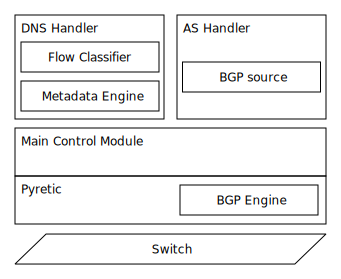
\epsfig{file=./diagrams/architecture2, width=.8\columnwidth}
    \caption{\system{} architecture}
    \label{fig:architecture}
\end{figure}


\system{} is SDN-based system running on Pyretic.\cite{pyretic} %and works on top of the SDX platform~\cite{sdx}. %This provides easy to understand syntax for network operators.
\system{} is divided into three parts, as can be seen in Figure~\ref{fig:architecture}. There are two monitoring modules, described below, that provide traffic identification and monitoring information to the main control module (MCM). %The MCM is responsible for combining information from the classification modules and, based on the network operator's policies, writing rules into the network switches.%It is a layer on top of the SDX platform.
The MCM is responsible for combining the results from the monitoring modules, and implementing the reactive policies defined by the network operator.

%In the examples above, the MCM would be responsible for integrating the resulting policies low level policies from the DNS handler and AS handler for the \tti{traffic\textunderscore{}in\textunderscore{}bytes()} and \tti{match\textunderscore{}AS()} and sending the matched flows or packets to the the \tti{rate\textunderscore{}limit()} and \tti{drop()} actions.


\subsection{DNS Handler}
The DNS handler contains two parts, a flow classifier based on part of FlowQoS~\cite{FlowQoS} and a metadata engine. %The metadata engine requires the flow classifier, but the flow classifier can be used as a standalone module. In fact, the flow classifier is based on a part of FlowQoS~\cite{FlowQoS}, but is entirely rewritten and heavily enhanced.

To perform flow classification, two pieces of information are needed: URL-to-classification mapping and IP-to-URL mapping. The URL-to-classification mapping is mentioned above where \tti{googlevideo.com} maps to `video'. This is a manual lookup, implemented as regular expression matching. The IP-to-URL mapping is based on monitoring DNS responses. At intialization, rules are installed at all ingress network devices to make a copy of DNS responses, forward one to the actual destination, and forward the second to the DNS handler. The flow classifier then expracts the domains and associated IP addresses, and uses the URL-to-classification mapping to determine what type of traffic is associated with a particular IP address. 

%At startup, the DNS handler creates a rule in all ingress network devices to make a copy of DNS responses, forward one to the actual destination, and forward the second to the DNS handler, and to the flow classifier in particular. The flow classifier parses the DNS packet, extract the domains and associated IPs, and classifies traffic from the IPs based on the domain name. 

The metadata engine handles policy implementation for DNS-based classification. The metadata engine is responsible for breaking down the high-level policies passed form the MCM into the constituent components, and handling any changes that my occur dynamically (\ie{}, when a new DNS response comes in, or DNS response time-to-live (TTL) is reached). It is also responsible for aggregating data, such as aggregating the number of bytes transferred by video sources.

To go over the example above, if during the example above a DNS response from \tti{googlevideo.com} with associated IP of 198.51.100.8 was seen, the URL will be classified as video, and, as such, traffic coming from 198.51.100.8 would be classified as video. This will cause the \tti{matchClass} policy to generate a new \tti{match} action to run in parallel with any preexisting actions associated with video traffic. 

\begin{comment}
% Continuing with our video example, if a policy is written to calculate how much video traffic is coming into a network, the metadata engine is responsible for breaking down the high-level policy passed from the MCM into the constituent components. That is, for each new IP address associated with the video classification, it is responsible for creating byte-counter rules for each IP, then aggregating the values reported, and returning this information to the MCM.

% In the first example in section~\ref{sec:examples}, the new DNS response from \tti{googlevideo.com} would cause the metadata engine to create a new byte counter for flows between 198.51.100.8 and Bob's PC. The new counter would be added to the previous policy and added to any prior video byte counter aggregation. The total would be passed up the the MCM to make any decisions based on the total amount of video traffic to Bob's PC.

%The flow classifier has two main components. The first is the DNS-to-classification database. It contains mappings of IP addresses to classifications, along with metadata about the mapping - the DNS lookup string, expiration time, and the time-to-live (TTL) value from the DNS server. The second component is the DNS parser. This performs two actions, making DNS queries (requested by the metadata engine), and parsing all DNS responses, from self-issued requests and from network user requests.

%The metadata engine is the interface to the policies of \system{}. Going back to our video example, when a new DNS entry comes into the flow classifier, and a classification is assigned, the metadata engine looks at it. If it is classified as `video', the metadata engine will push a new rule to create counters per user to the switches.
\end{comment}

\subsection{AS Handler}
To allow for rules based on traffic related to a particular AS, BGP information is necessary. \system{} uses an external source of BGP information. This could be a connection to a local BGP server, or could be a static database of known routes. The BGP information source plays a similar role to the Flow Classifier in the DNS handler: it provides a lookup source for AS routes, and, more importantly, ranges of addresses controlled by a particular AS.

Since BGP routes can update dynamically, the AS Handler handles these updates in much the same way as the BGP Handler handles expiration of DNS information. This allows for implemention the aforementioned security policy wherein ASes on blacklists can have their traffic redirected to a security appliance easily.

\begin{comment}
As \system{} is based on the SDX platform which contains a BGP-engine, we have access to BGP routes. The primary responsibilities are similar to those of the DNS handler, in that the AS handler needs to break down the high level policy into its constituent components and returning them to the MCM.
%In the case where a network operator wants to send all traffic from a particular AS to a virus scanner appliance, the AS handler will identify which IP addresses are associated with the specified AS, and return these to the MCM. The MCM can then route the traffic vide the virus scanner appliance.

In the second example from section~\ref{sec:examples}, the AS handler would be responsible for breaking down the \tti{match\textunderscore{}AS()} into the constituent components. These components would be a series \tti{match()} actions on source IP addresses from packets to the IP ranges that AS~12345 was advertising. The parallel composition of all of these \tti{match()} would be composed with the \tti{drop()} action by the MCM.

%the AS Handler will install rules for all traffic originating from that AS's advertised IP address blocks. If the network operator does not trust any traffic that passes through a particular AS, the AS Handler can install rules for any IP address block where the AS is in the AS-Path of the BGP route.

Many networks, in particular home or small business networks, BGP information is not accessible. As such, this handler can be seen as optional.
\end{comment}


%%%\subsection{Data Flow}
%Rules are installed at startup of \system{}, so anything that happens subsequently is dynamic. In particular, the DNS and BGP bindings will change, expire, and be repopulated regularly. As such, we will describe a flow for the first example in the previous section.

%At initialization, multiple rules will be created. First, byte count rules for traffic classified as video destined for Bob's PC will be installed. These counts will be reported at a set interval (perhaps once per minute). As category-specific rules are DNS-based, each of the different video counting rules will be summed by the DNS metadata engine and reported to the MCM.

%As Bob visits different video websites, DNS requests will be made by his PC. The responses will be inspected by the DNS flow classifier, while simultaneously forwarding the response to Bob. When Bob does request the video, the source IP will be checked by the DNS metadata module against the DNS database to find out if it has been classified. Since it is a video source, new byte counter rules for the new flow will be installed, and added to the previous rules. 

%Once the 10 gigabyte limit is hit, the MCM will create a \tti{ratelimit} rule and write that to the closest switch to Bob's PC.

%%This section will go into detail of the inner workings of the first example above, about limiting Bob's video consumption. We are only going to discuss the actions of the DNS handler, but the actions of the AS handler will be substantially the same.

%%%Policy is established at startup of \system{}, so anything that happens subsequently is dynamic. In particular, the DNS and BGP bindings will change, expire, and be repopulated regularly. We will now describe part of the behavior of the first example, limiting Bob's video consumption. We are only going to discuss the actions of the DNS handler, but the actions of the AS handler will be substantially the same.

%%%When a new DNS response comes in, the response is parsed and classified. If it is classified as video, the DNS metadata engine will create new rules that establishes byte counters for Bob's PC to all traffic coming from the IP addresses associated with the video site. It does not matter if Bob was associated with the DNS request, the rules would be installed regardless.

%%%There are likely multiple addresses associated with video traffic, and likely as many counters. These counters will need to be accumulated, which is also handled by the DNS metadata engine. The total of the counters is sent to the MCM, which, if the total has reached 10 gigabytes for the month, will create a \tti{ratelimit} rule and write the rule to the closest switch to Bob's PC.

